% !TEX root = ccsn.tex
\section{Detection sensitivity with Advanced gravitational wave detectors}
\label{sec:results}

\begin{figure}[t]
 \centering
 \includegraphics[width=0.5\textwidth]{plots/spectrum}
 \caption{Amplitude spectral density of the GW detectors aLIGO and AdV at design sensitivity and that of the proposed third-generation detectors Cosmic Explorer and Einstein Telescope. Einstein Telescope sensitivity curve ET-B is obtained pushing second-generation detector technology at its limit. ET-C and ET-D sensitivity curves correspond to a detector configuration where a low-power cryogenic low-frequency interferometer and a high-power room temperature high-frequency interferometer are sharing the same infrastructure~\cite{Hild_2011}. Cosmic Explorer design sensitivity will be achieved in two stages. Stage 1 (CE1) is expected to use the technology developed for the ``A+'' upgrade to aLIGO but scaled up to a 40 km detector while stage 2 (CE2) will implement state-of-the-art technology to decrease quantum and thermal noises~\cite{reitze2019cosmic}. } \label{fig:spectrum}
\end{figure}

\begin{figure}[t]
  \centering
  \begin{tabular}{c}
    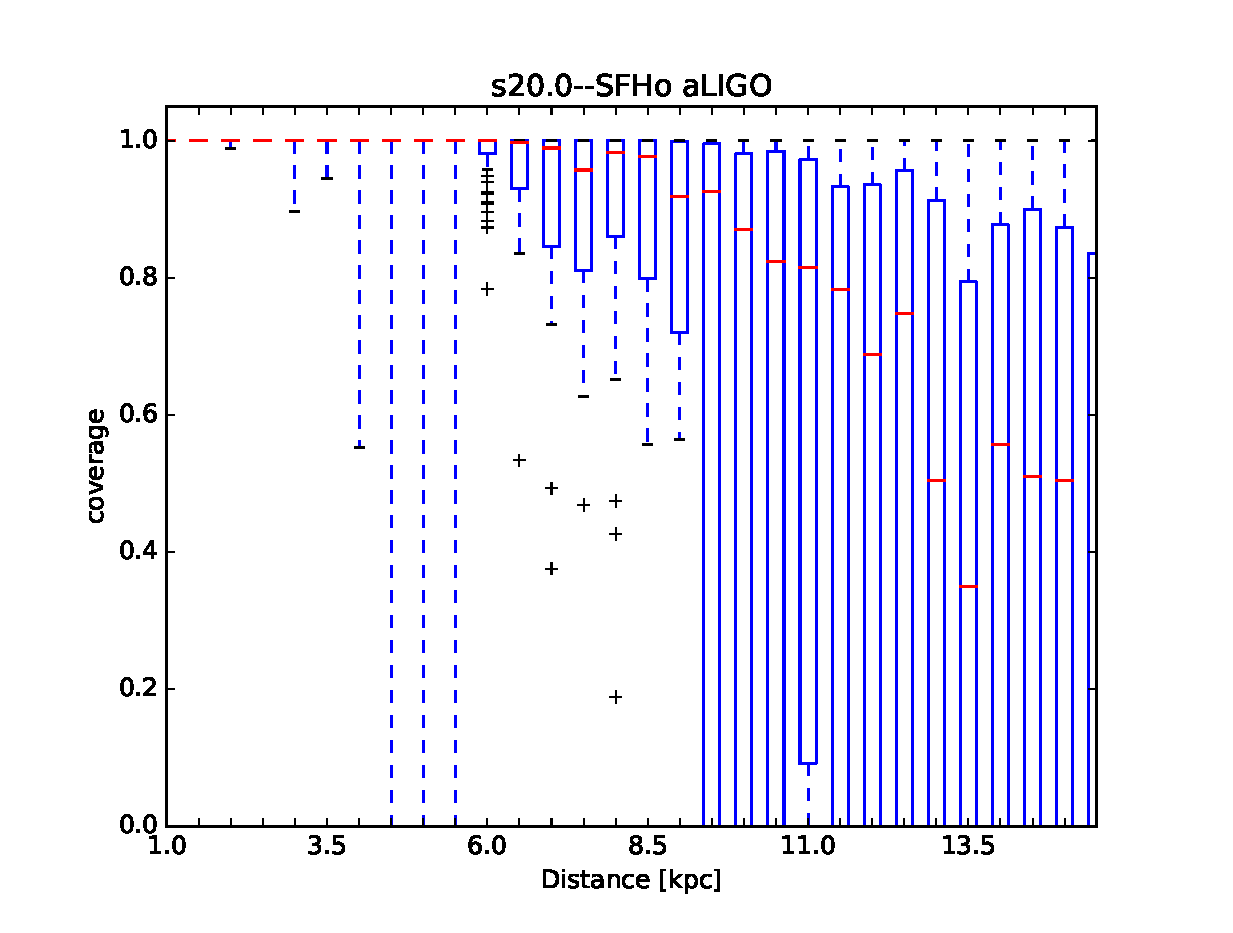
\includegraphics[width=0.5\textwidth]{plots/s20--SFHo_covpbb_boxplot_aLIGO} \\
    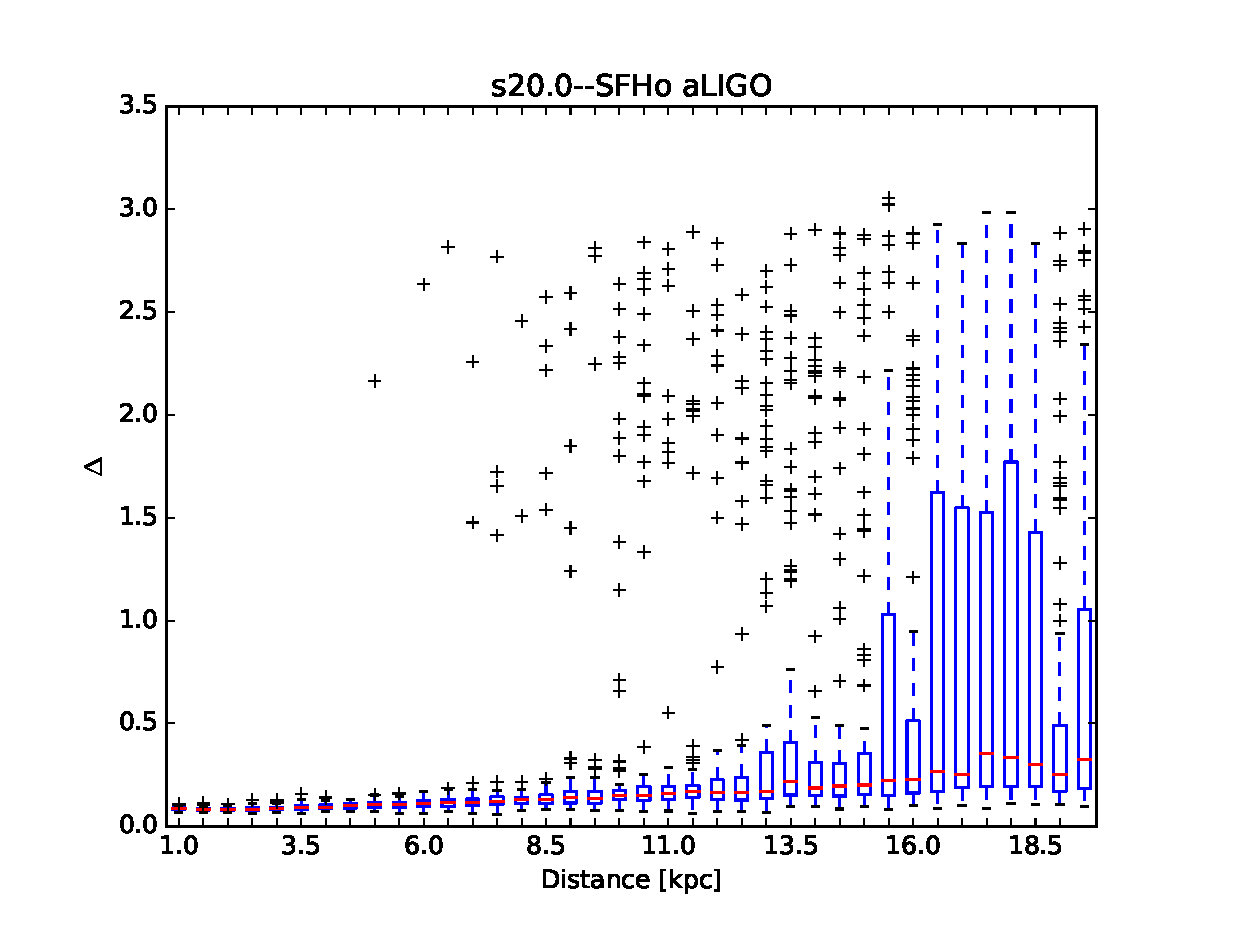
\includegraphics[width=0.5\textwidth]{plots/s20--SFHo_error_boxplot_aLIGO} \\
  \end{tabular}
    
 \caption{Boxplots of the $coverage$ (upper panel) and $\Delta$ (lower panel) for {\texttt s20S} signal embedded in aLIGO noise at different distances from the Earth. 100 noise realizations are considered for each distance. \tf{We should explain a bit more the symbols and colours that appear in the plots.}}
  \label{fig:s20results}
\end{figure}

\tf{We probably need a better title for this section.}

To estimate how accurately we can infer the time evolution of $r(t)$ in the GW data of a single
detector we inject the GW signal for model {\texttt s20S} into 
100 Gaussian noise realisations whose power spectral density (PSD) follows the aLIGO
spectrum~\cite{aLIGOsens:2018}. The PSD of aLIGO and AdV at design sensitivities, along with those of planned third-generation detectors, are shown in Figure~\ref{fig:spectrum}. 

We cover a large range of distances for which a CCSN detection in second-generation GW detectors is feasible. We assume that the source is optimally oriented with respect to our single detector. Moreover, we also assume that a CCSN GW signal has been identified in the data and that the beginning of the signal is known within {$\mathcal O$}(10 ms). The data (signal embedded in noise) are whitened using the function {\tt prewhiten} of the R-package {\tt TSA}. An auto-regressive model with a maximum of maximal 100 coefficients is used.    

For each of the noise realizations we reconstruct the ratio time series {$r_i$} of length $N$ starting from the left side of the spectrogram and constraining the beginning of the track to be smaller than \unit[200]{Hz}. \tf{Perhaps we should mention that this value is chosen using the information on the initial mode frequency from the simulations.}
The reconstructed ratio is then compared to the ``true'' ratio {$r_i^0$} derived from the PNS mass and radius computed from the {\texttt s20S} simulation. The top panel of Fig.~\ref{fig:s20results} shows the distribution of the fraction of the ratio values {$r_i^0$} that fall within the 95\% confidence interval of {$r_i$} as a function of the distance to the source. This quantity, hence, gives information about the {\it coverage} of the reconstructed ratio. The coverage takes maximum values when the source is located within a few kpc and then decreases with the distance.

To better quantify how well we reconstruct the ratio we also consider  the mean of the relative error of $r_i$ along 
the track of the spectrogram, $\Delta$,  
\begin{equation}
\Delta=\frac{1}{N}\sum_1^N\frac{|r_i-r_i^0|}{r_i^0}\,.
\end{equation}
The values of $\Delta$ for each of the 100 noise realizations are shown as a function of the distance
in the bottom panel of Fig.~\ref{fig:s20results}. For a source located up to $\sim$\unit[9]{kpc} the relative error
remains smaller than 20\%. At closer distances $\Delta$ is smaller but it does not vanish. This reflects the approximate nature of the model used for $r$. It is nevertheless remarkable that, on average, one can reconstruct the ratio time series with a good
precision up to distances of $\sim$ 9 kpc (for this particular waveform) with a coverage value
larger than 80\%. We note that there are a few noise realizations for distances below 9 kpc for which
$\Delta$ takes large values, indicating that the method fails to accurately reconstruct the ratio in those case. \tf{Do we know why that is the case? What is intrinsically different from one noise realisation to another that makes the method more prone to failure? I think we should provide some explanation here, if we have it.}

\begin{figure}[t]
  \centering
  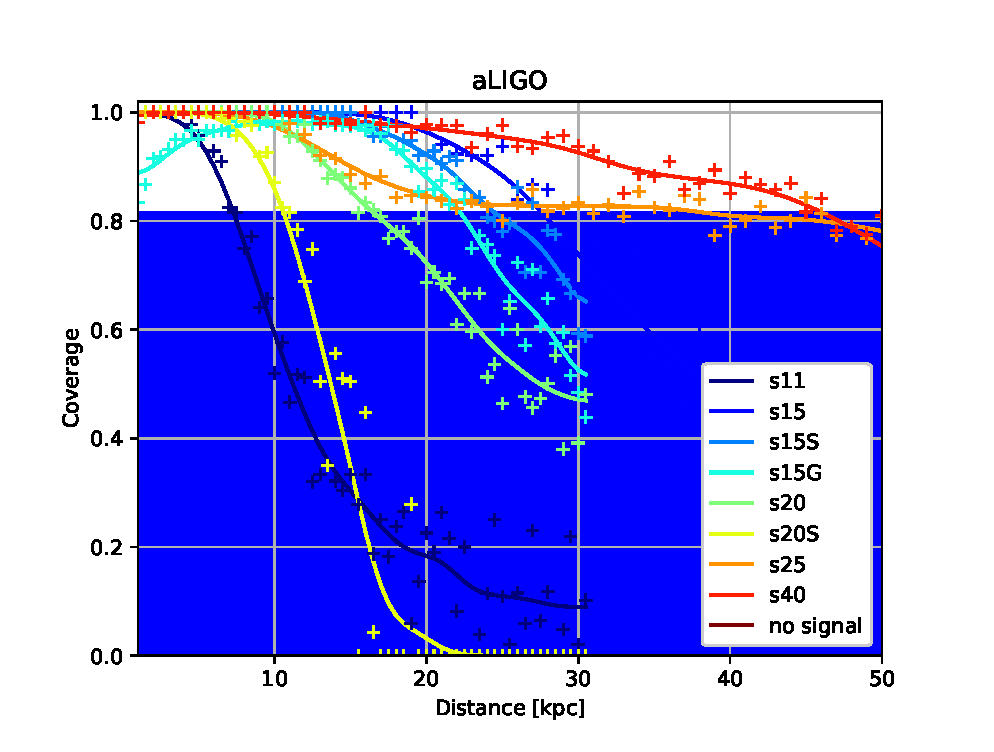
\includegraphics[width=0.5\textwidth]{plots/aLIGO_coverage_allwvfs}
 \caption{Median of the coverage for the eight CCSN waveforms of the {\it test set} embedded in aLIGO noise as a function of the  distance to the source. The ``no signal'' line and band show the median and first and third quartile of coverage in absence of any signal. The line of the latter is zero and overlaps with the horizontal axis (see main text for details). \tf{Perhaps is more consistent to use in the legend the same model names as in Table 1. Some of the colours are really hard to see, particularly for s20S. That could perhaps be improved if we use thicker lines. I'm confused about the quartiles shown.}} \label{fig:aLIGO_cov_allwvf}
\end{figure}

\begin{figure}[t]
  \centering
  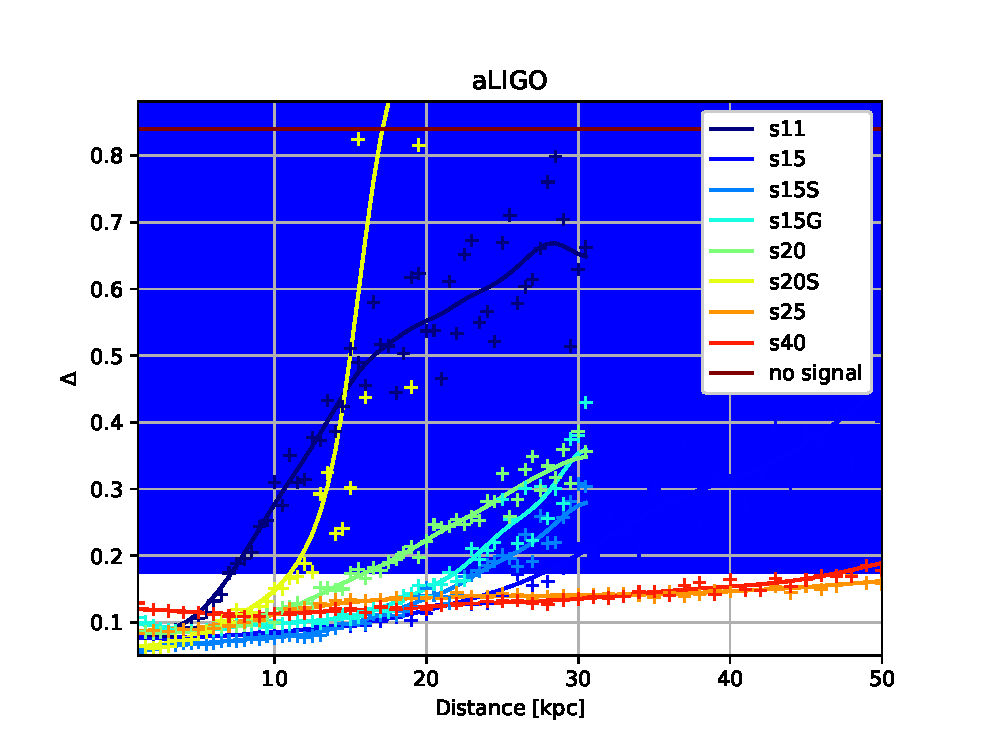
\includegraphics[width=0.5\textwidth]{plots/aLIGO_delta_allwvfs}
 \caption{Same as Fig.~\ref{fig:aLIGO_cov_allwvf} but for the relative error $\Delta$. \tf{Same comments as for Fig.~\ref{fig:aLIGO_cov_allwvf}.}}
% Median of $\Delta$ for 8 CCSN waveforms embedded in aLIGO noise and located at different distance from the Earth. The ``no signal'' line and band show the median and first and third quartile of $\Delta$ in absence of any signal.} 
\label{fig:aLIGO_prec_allwvf}
\end{figure}

We have tested that the method does not depend on the specific features of the waveform of model {\texttt s20S} by repeating the procedure for the remaining seven waveforms of the {\it test set} described in Section \ref{sec:simulations} covering
a large range of progenitor masses. Figure \ref{fig:aLIGO_cov_allwvf} shows that apart from model {\texttt s11} and to a lesser extent model {\texttt s20S}, the ratio is well reconstructed for all waveforms up to a distance of $\sim$ 15kpc. In an
effort to better determine the maximal distance of the source at which we can reconstruct the ratio we have run 100 simulations without injecting a signal and have measured the corresponding coverage for the reconstructed ratios.
The median of the coverage as well as the 95 quartile are shown in Figure \ref{fig:aLIGO_cov_allwvf}. \tf{This seems inconsistent with what is written in the caption, which indicates the third quartile.}
The noise only median value is identically zero in this case. However, note that it could be different from zero because
the g-mode reconstruction algorithm is looking for a continuously  increasing frequency track
in the spectrogram, starting between 0 and 200 Hz, where we expect the GW signal to be.
This is enhancing the probability of overlap. This effect explains why outliers can reach
values as high as 80\%. \tf{I don't understand this last comment.}

Figure \ref{fig:aLIGO_prec_allwvf} shows the relative error $\Delta$ as a function of the distance for the signals of the {\it test set}
as well as the result when only noise is considered. This quantity follows the same trend than that followed by the coverage, since all signals but models {\texttt s11} and {\texttt s20S} are reconstructed with relative errors below 20\% up to distances of $\sim$ 15kpc. Correspondingly, the no-signal case yields the largest error, as expected.

We perform the same analysis using the design sensitivity curve of AdV and expected sensitivity curves for the third-generation 
GW detectors. The results for the former are reported in Table \ref{tab:results}. We focus now on third-generation detectors whose results are reported in Table \ref{tab:results} and shown in Fig.~\ref{fig:s20--SFHo_all3G}. In Europe the Einstein Telescope project proposes to host in a 10-km equilateral triangle configuration three low-power low-frequency cryogenic interferometers as well as three high-power high-frequency interferometers. Three sensitivity curves, ET-B, ET-C and ET-D corresponding to different options and stages of the project~\cite{Hild_2011} are considered in our study (cf.~Fig.~\ref{fig:spectrum}). The US based project Cosmic Explorer~\cite{reitze2019cosmic} is expecting to reach its design
sensitivity circa 2040 through two phases labeled CE1 and CE2, whose sensitivity curves are also shown in Figure~\ref{fig:spectrum}. 

%%%


Table \ref{tab:results} reports the source distances $d_r$ in kpc at which the median of the coverage is lower than 95\% of the noise only values for aLIGO, AdV, and different configurations of third-generation detectors. We have checked that using either the median of the coverage or the median of $\Delta$ yield similar results for the distance.
The numbers on the table are an estimate of the order of magnitude of the source maximal distance at which a
reconstruction of the ratio could be possible with current and planned GW detectors.
They are also upper limits as we are taking into account the detector antenna response in our
simulation but assume that the source is optimally oriented with a matched filter signal-to-noise ratio of 13. 
Table \ref{tab:results} shows that the results for the Advanced Virgo detector at design sensitivity are very similar to those of aLIGO, despite the differences in detector sensitivity.
%Note that Table \ref{tab:results} provides the distance at which one could detect a source
%optimally oriented with a matched filter signal-to-noise ratio of 13.







Figure \ref{fig:s20--SFHo_all3G} shows $\Delta$ as function of the source distance for {\texttt s20S}
waveform for the five third-generation detector configurations we analyze. Overall, the ratio is well reconstructed up to distances
in the range \unit[100--200]{kpc} which represents an improvement of a factor 10 with respect to
Advanced LIGO and Advanced Virgo detectors. We can also note that the Einstein Telescope results lay in
between the 2 Cosmic Explorer results. This is confirmed for all other waveforms, expect {\texttt s25}
for which the maximal distance reach in CE2 is significantly lower than CE1. This is partly due to the
small variation of the reconstruction quality to the distance of the source making the estimation of $d_r$
rather uncertain for this waveform. All results are summarized in Table \ref{tab:results} and Figure
\ref{fig:distances}. It is remarkable that with 3G detectors the ratio could be reconstructed for sources
located up to several hundred of kpc. It is nevertheless important to note the rather wide range obtained
for the different waveforms probing a large range of progenitor masses.
We did not find any correlation between the mass of the progenitor and $d_r$, nor the equation of state.
On the other hand, the quality
of the ratio reconstruction depends on the signal-to-noise ratio, expressed in Table \ref{tab:results} by
$d_{det}$.

\begin{figure}
  \centering
  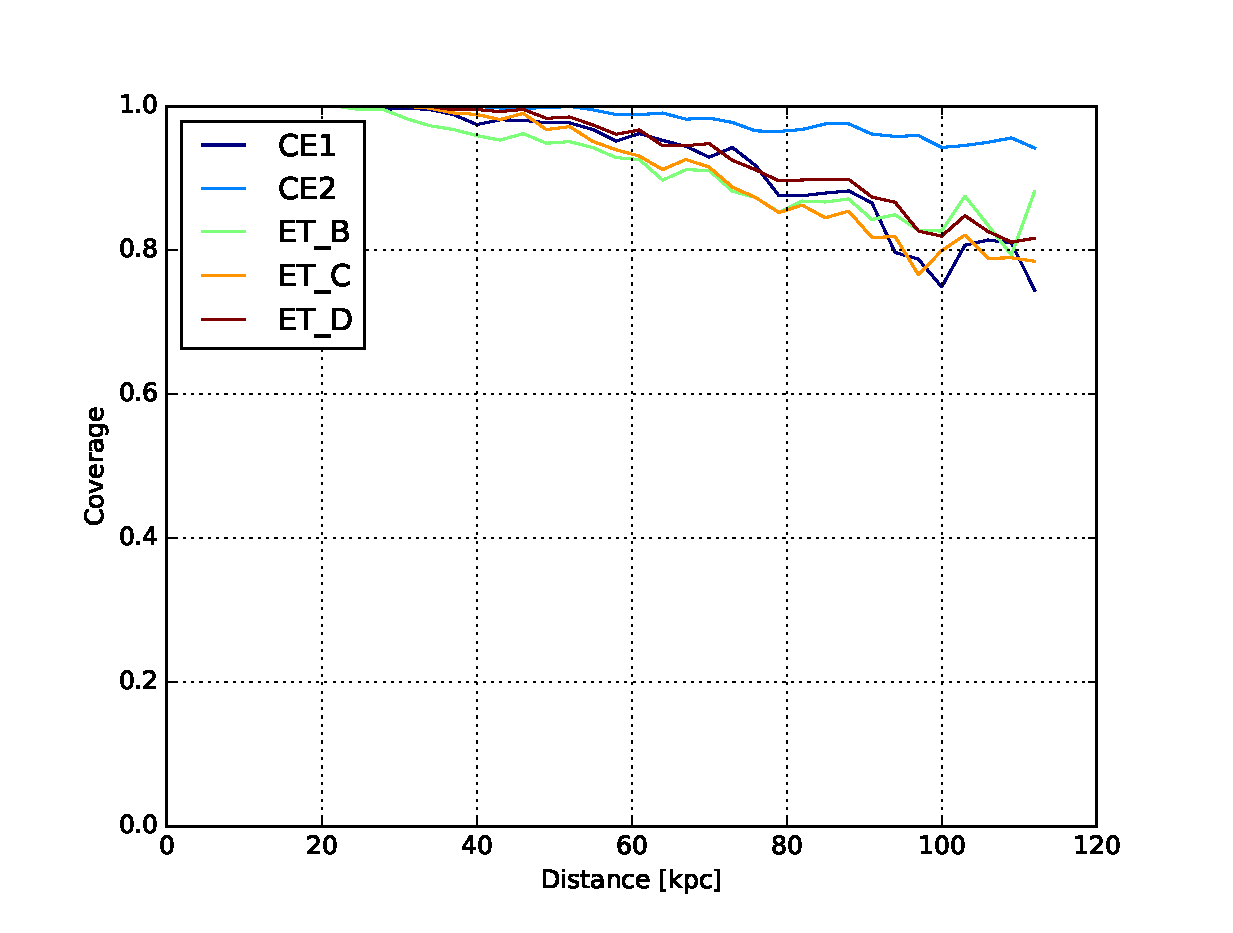
\includegraphics[width=0.5\textwidth]{plots/s20--SFHo_all3G}
  \caption{Median of $\Delta$ for {\texttt s20S} CCSN waveform embedded in 3G detectors noise and located at different distance from the Earth. } \label{fig:s20--SFHo_all3G}
\end{figure}

\begin{figure}
  \centering
  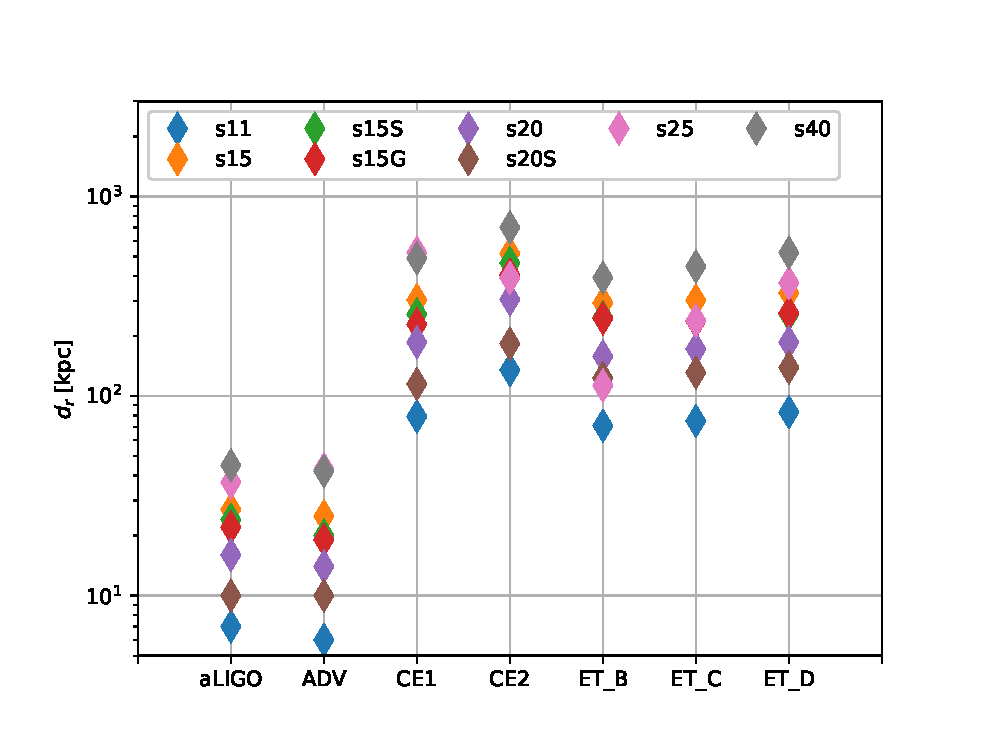
\includegraphics[width=0.5\textwidth]{plots/dist_allwvfs_2G3G}
  \caption{Maximal distance $d_{r}$ in kpc at which the ratio $r=M_{\rm PNS}/R_{\rm PNS}^2$ is reconstructed
    with good accuracy for a source optimally oriented with respect to the GW detectors for the 7 CCSN waveforms considered in this study.} \label{fig:distances}
\end{figure}



\begin{table}
  \centering
  \begin{tabular}{c|c|cccccccc}

\multicolumn{2}{c|}{}  & \texttt{s11} & \texttt{s15} & \texttt{s15S} & \texttt{s15G} & \texttt{s20} & \texttt{s20S} & \texttt{s25}  & \texttt{s40}\\   

\hline
\multirow{3}{*}{aLIGO} & $d_{r}$   & 7 & 28 & 24  & 22 & 16 & 11 & 38 & 46 \\
\cline{2-10}
                       & $d_{det}$ & 11 & 36 & 26 & 27 & 21 & 16 & 74 & 61\\
%                      & SNR      & 14 & 46 & 33 & 35 & 27 & 21 & 96 & 80\\

\hline
\hline
\multirow{3}{*}{ADV}   & $d_{r}$   & 7  & 26  & 20 & 19 & 15 & 10 & 43 & 42 \\
\cline{2-10}
                       & $d_{det}$ &  10 & 32 & 22 & 23 & 18 & 13 & 64 & 52\\
%                      & SNR      &  13 & 41 & 29 & 30 & 23 & 17 &  83 & 68\\

\hline
\hline
\multirow{2}{*}{CE1}   & $d_{r}$   & 79  & 304 & 258 & 229 & 187 & 115 & 524 & 490 \\
\cline{2-10}
                       & $d_{det}$ & 115 & 377 & 270 & 282 & 217 & 168 & 774  & 633\\
%                      & SNR      & 149 & 490 & 352 & 366 & 282 & 218 & 1006 & 822\\

\hline
\multirow{2}{*}{CE2}   & $d_{r}$  & 135 & 499 & 451 & 405 & 305 & 183 & 391 & 898 \\
\cline{2-10}
                       & $d_{det}$ & 197 & 649 & 468 & 489 & 375 & 294 & 1347  & 1100\\
%                      & SNR    & 256 & 843 & 608 & 635 & 487 & 382 & 1751 & 1430\\

\hline
\multirow{2}{*}{ET\_B} & $d_{r}$ & 71  & 293 & 248 & 245 & 158 & 123 & 113 & 392 \\
\cline{2-10}
                       & $d_{det}$ & 106 & 364 & 274 & 391 & 216 & 200 & 805 & 665\\
%                      & SNR      & 138 & 473 & 356 & 379 & 381 & 260 & 1046 & 865\\

\hline
\multirow{2}{*}{ET\_C} & $d_{r}$ & 75  & 302 & 239 & 237 & 172 & 131 & 239 & 446 \\
\cline{2-10}
                       & $d_{det}$ & 97 & 332 & 246 & 260 & 194 & 164 & 727  & 603\\
%                      & SNR      & 126 & 432 & 320 & 338 & 252 & 213 & 945 & 783\\

\hline
\multirow{2}{*}{ET\_D} & $d_{r}$ & 83  & 329 & 257 & 261 & 186 & 139 & 369 & 523 \\
\cline{2-10}
                       & $d_{det}$ & 107 & 368 & 271 & 285 & 213 & 174 & 796  & 661\\
%                      & SNR      & 140 & 477 & 352 & 371 & 277 & 227 & 1034 & 859 \\

  \end{tabular}
  \caption{%%
    Maximal distance $d_{r}$ at which the ratio $r=M_{\rm PNS}/R_{\rm PNS}^2$ is reconstructed
    with good accuracy for a source optimally oreinted with respect to the GW detectors
    considered in this study. $d_{det}$ is the distance at which one could detect a source
    optimally oriented with a matched filter signal-to-noise ratio of 13 in the  different
    GW detectors. All distances are expressed in kpc.
    %%
  }
  \label{tab:results}
\end{table}

